
\chapter{Introduction}
\label{cha:1_Introduction}

% the code below specifies where the figures are stored
\ifpdf
    \graphicspath{{1_introduction/figures/PNG/}{1_introduction/figures/PDF/}{1_introduction/figures/}}
\else
    \graphicspath{{1_introduction/figures/EPS/}{1_introduction/figures/}}
\fi


%-------------------------------------------------------------------------
%Chapter 1 contents:
%- Motivation of the research field: Context-aware systems -> LBS -> GNSS limitation -> Positioning techniques -> DR -> inertial PDR -> inertial PDR + wearables
%- Problem identification: smartphone not a wearable -> potentiality of wrist-worn wearables -> Problem: no wrist-worn PDRS
%- Goal of the thesis: tackle the problem -> how? Splitting it into sub-problems
%- Structure of the thesis
%-------------------------------------------------------------------------

Governments and companies are producing vast streams of data and require effective data analytics and machine learning methods to assist in making predictions and decisions promptly. One crucial aspect is the machine learning pipeline, which involves training a prepared dataset to construct a model and subsequently utilizing this model to predict new instance outputs. As depicted in Fig. \ref{fig:machine-old-senario}, the process entails fetching historical data from the database during the training phase to construct the machine learning model. Then, the system can input new instances from the database to predict the output.

\begin{figure}[!ht]
    \centering
    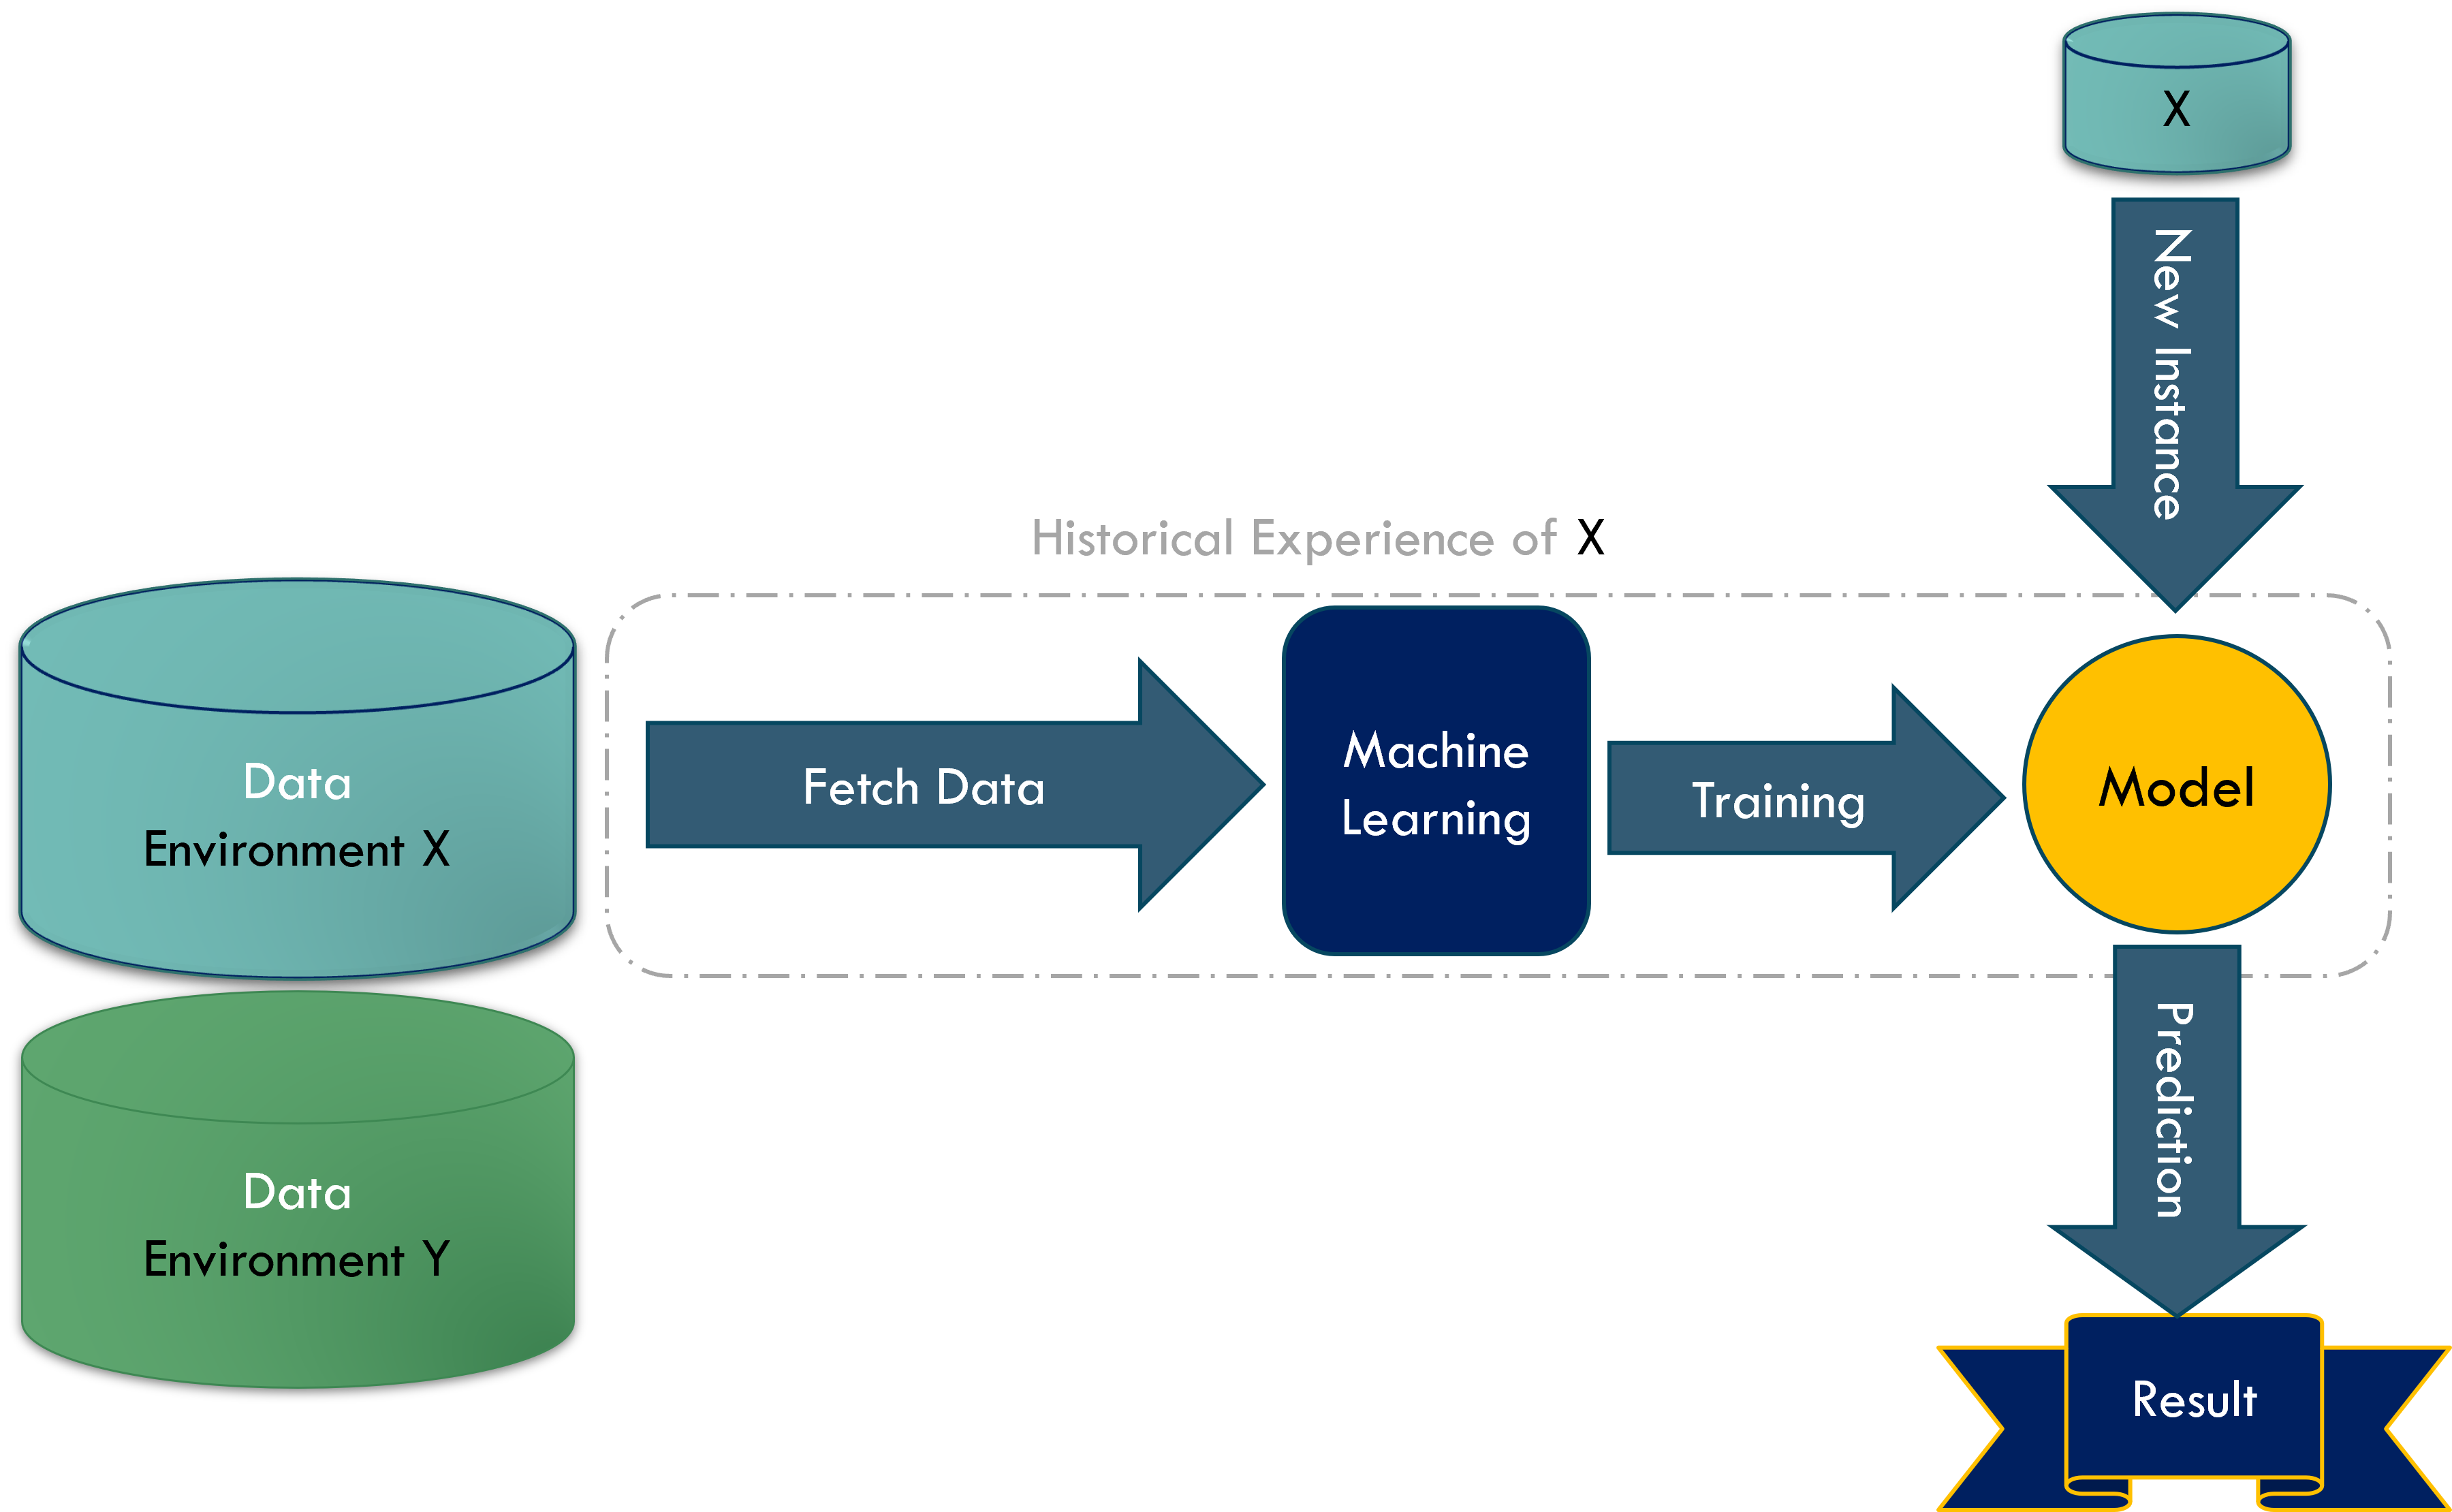
\includegraphics[width=.9\textwidth]{1_introduction/figures/PNG/machine_flow.png}
    \caption{Machine learning workflow for environment X.}
    \label{fig:machine-old-senario}
\end{figure}

Nevertheless, when endeavoring to forecast outcomes for fresh instances sourced from an alternative database, as illustrated in Fig. \ref{fig:machine-new-senario}
, there frequently emerges a conspicuous decline in accuracy. This disparity accentuates the imperative for model developers to intervene and rectify the issue. Addressing this, developers must adjust and retrain the model utilizing datasets from the new environment to ameliorate accuracy. This iterative process aims to refine the model's precision and ensure its efficacy across diverse contexts, thereby bolstering the reliability of decision-making and predictive capabilities. To confront this challenge, the field of auto machine learning endeavors to facilitate online updates to the model without necessitating direct intervention from developers for modification.

\begin{figure}[!ht]
    \centering
    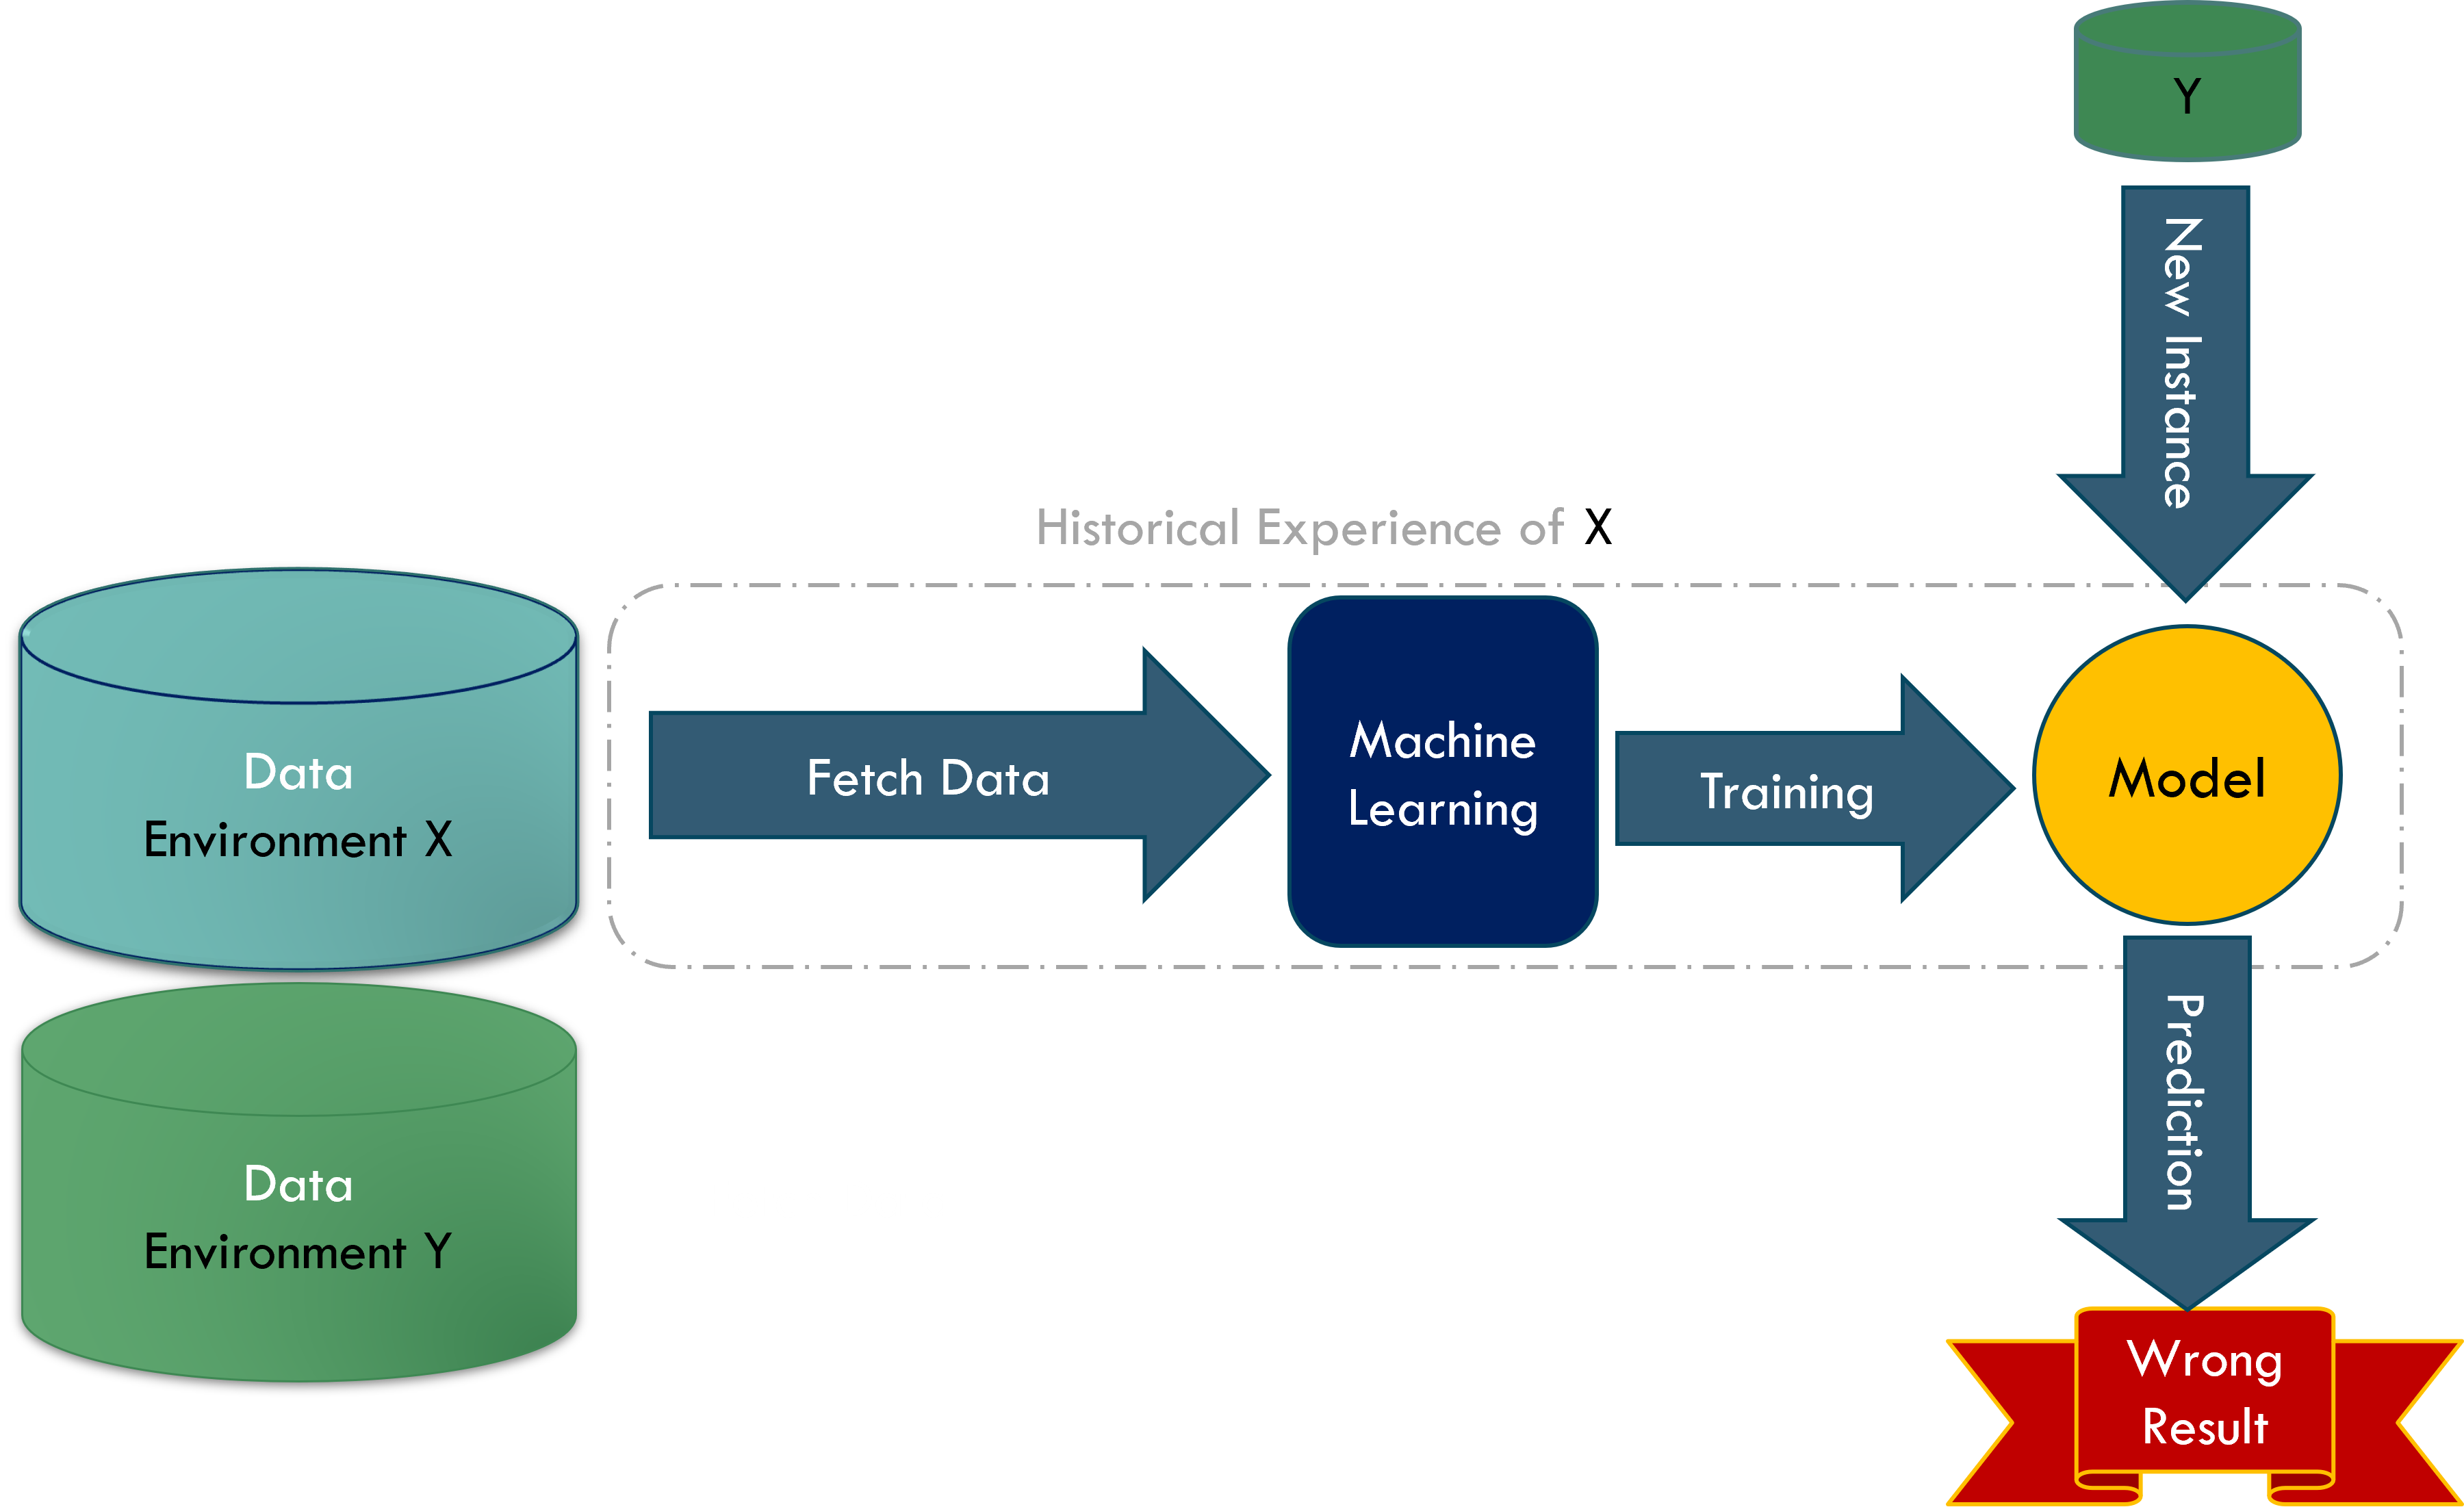
\includegraphics[width=.8\textwidth]{1_introduction/figures/PNG/wrong_machine_flow_1.png}\\
    (a) \\
    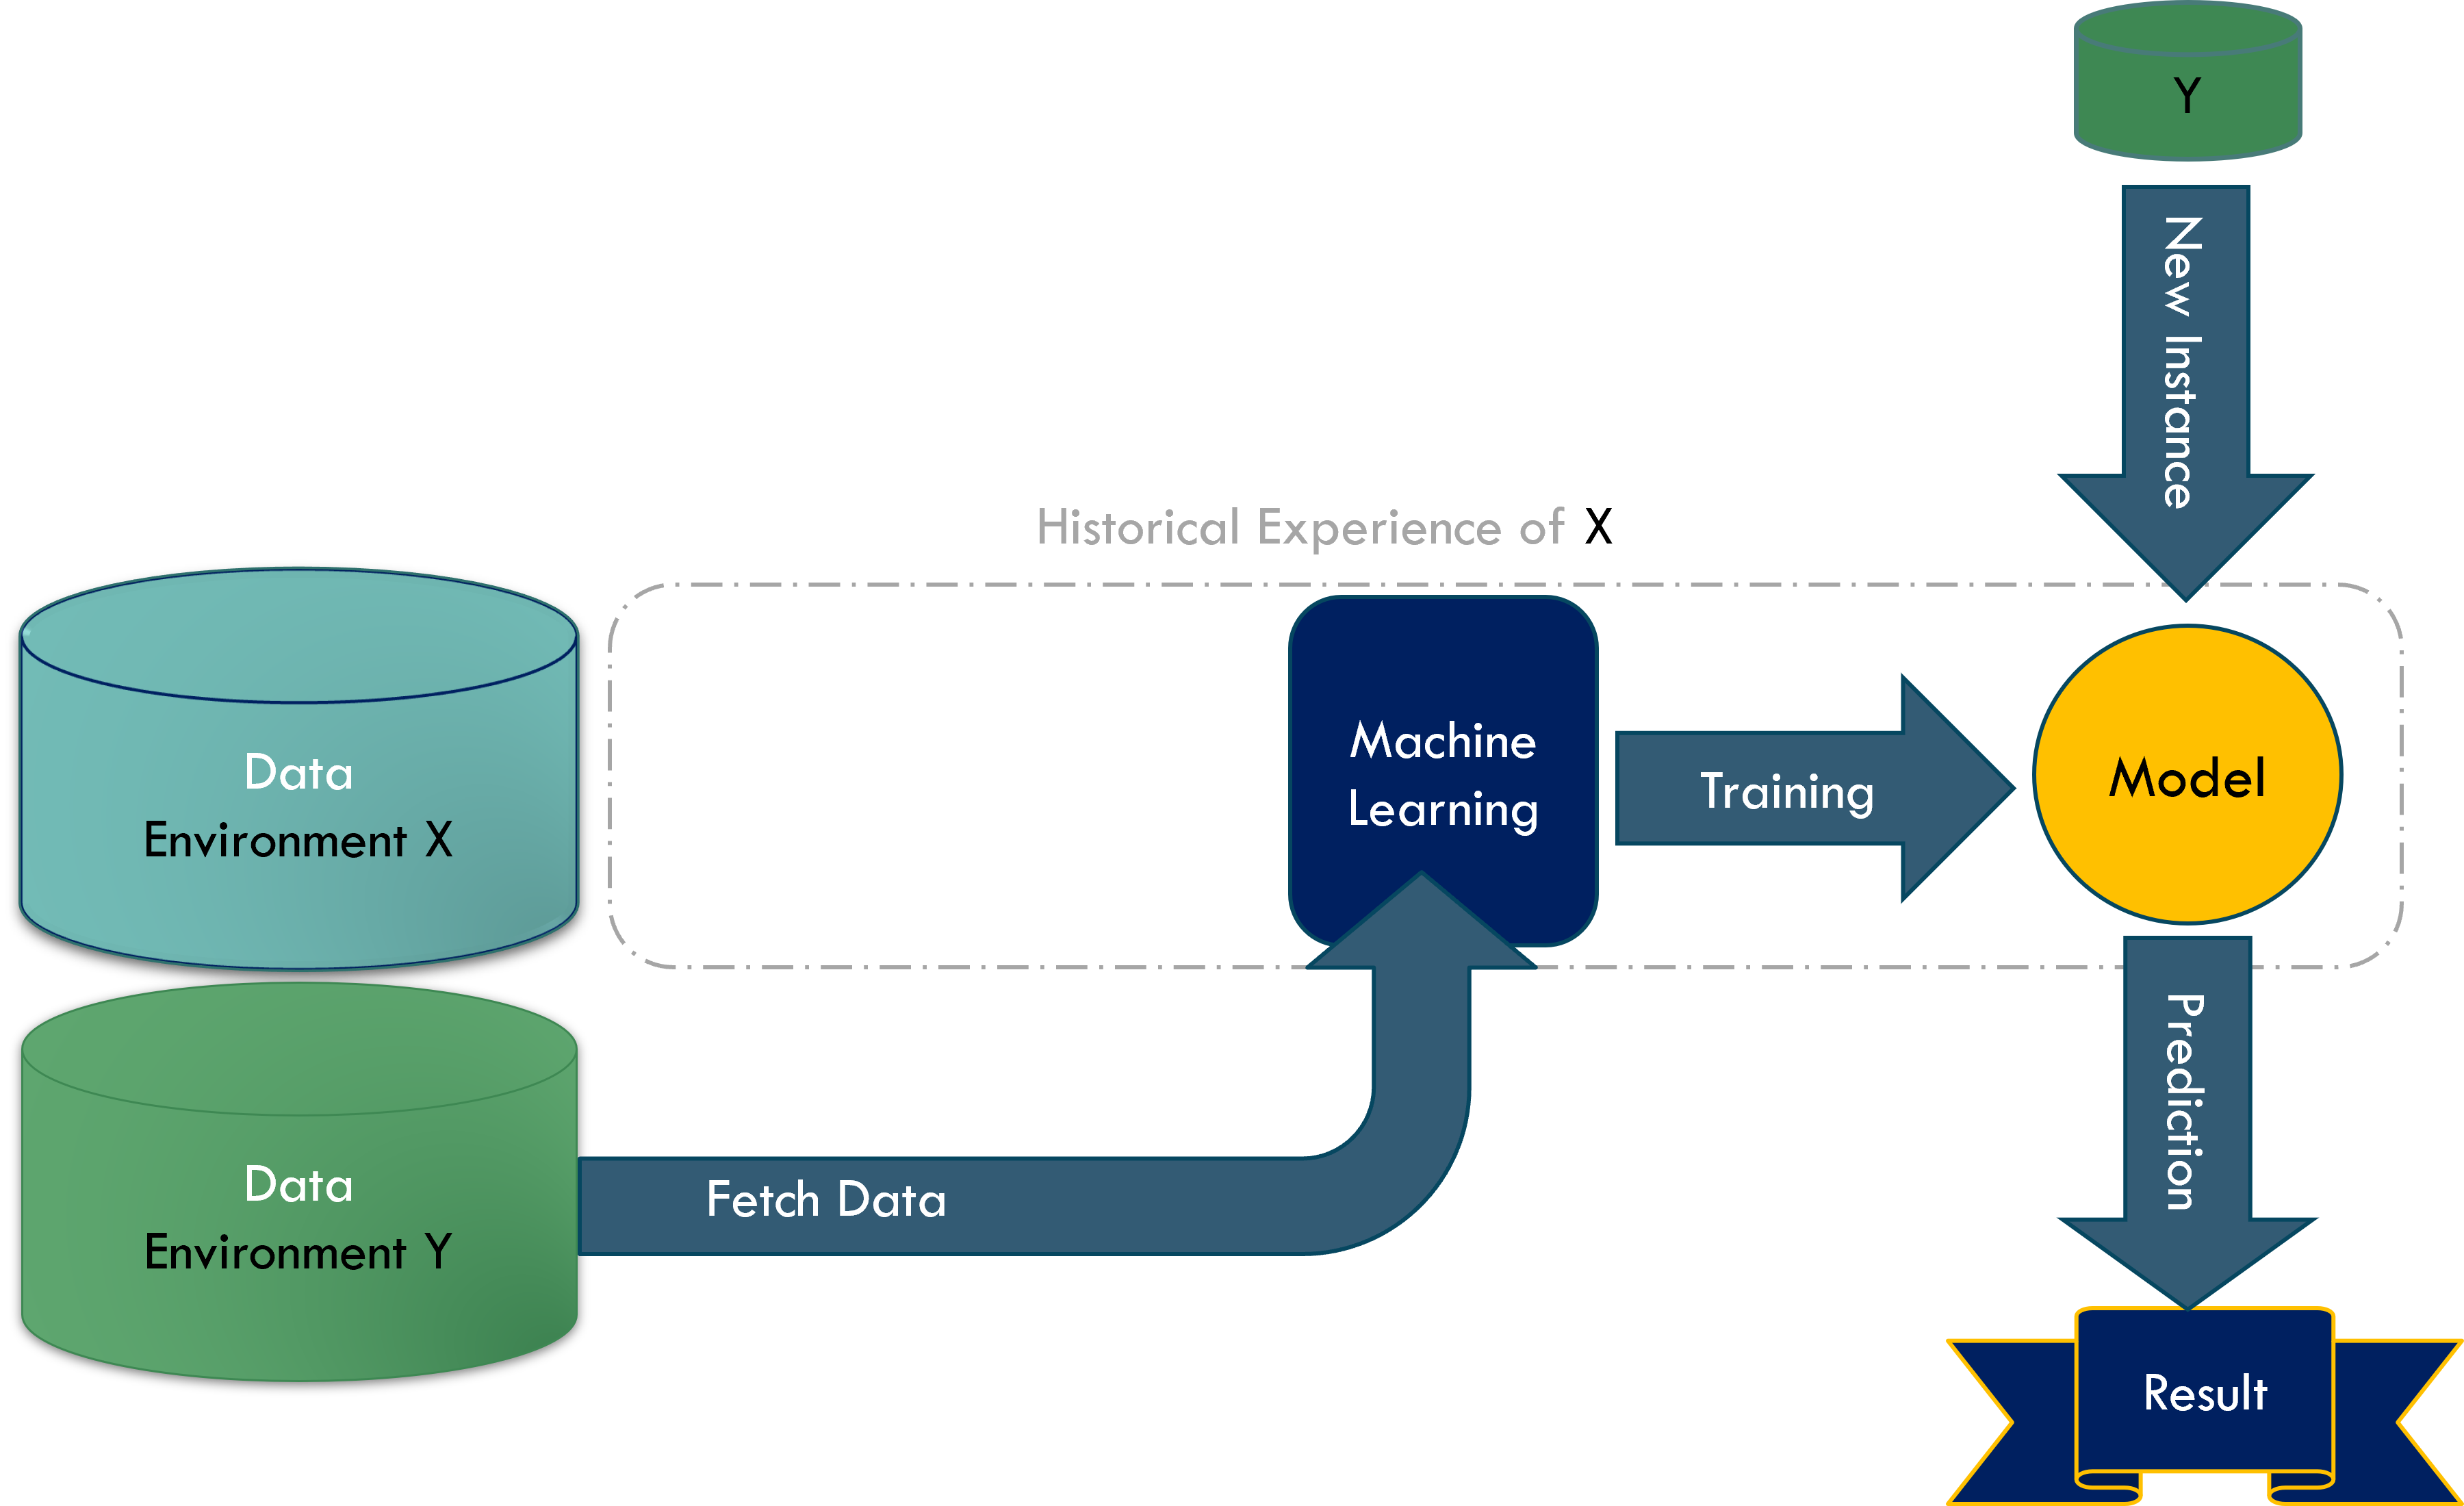
\includegraphics[width=.8\textwidth]{1_introduction/figures/PNG/wrong_machine_flow_2.png}\\
    (b)
    \caption{Machine learning workflow for environment Y.}
    \label{fig:machine-new-senario}
\end{figure}



In recent years, the surge in high-speed data streams has posed notable challenges for machine learning models, particularly in the context of streaming data analysis. These data streams, characterized by continuous, dynamic, and high-volume data arrivals, demand adaptive learning algorithms that can effectively cope with their evolving nature \cite{yang2021concept} \cite{dong2019multistream} \cite{shan2018online}. Within these evolving data environments, two paramount challenges have emerged: concept drift, class imbalance, Emerging new class, and heterogenous transfer learning.

Concept drift, a phenomenon defined by the evolving statistical properties of a data generation process over time \cite{pan2009survey} \cite{zhuang2020comprehensive}. introduces a dynamic element to the data, necessitating continuous adaptation of machine learning models. This shift can manifest as changes in underlying concepts, relationships between variables, or alterations in data distribution. Traditional models trained on historical data may suffer diminished accuracy or become inadequate when confronted with new data influenced by concept drift, highlighting the need for effective concept drift detection mechanisms. Addressing concept drift involves the utilization of concept drift detectors, which are methods capable of identifying changes in data stream distributions. These detectors rely on information related to classifier performance or incoming data items to signal the need for model updates, retraining, or even replacing the old model with a new one. The dynamic nature of concept drift necessitates ongoing monitoring and adaptation to maintain the model's efficacy.

Data streams also present challenges related to class imbalance, a condition characterized by uneven distribution among different classes \cite{wang2018systematic} \cite{sun2009classification}. This scenario, especially prevalent in multi-class settings, poses a significant challenge for traditional classifiers. The risk of misclassifying minority class samples due to their limited representation demands specialized techniques to ensure accurate classification without sacrificing the performance of the majority class \cite{charte2015addressing} \cite{charte2015mlsmote} \cite{daniels2017addressing} \cite{liu2018making}. To tackle class imbalance, three primary methods are commonly employed: sampling methods, algorithm adaptation methods, and hybrid methods. Sampling methods involve undersampling the majority class or oversampling the minority class to balance class distribution. Algorithm adaptation methods modify existing algorithms to handle imbalanced data \cite{japkowicz1995novelty} \cite{lopez2012analysis} \cite{zhang2020towards}, while hybrid methods combine data preprocessing with classification techniques, often utilizing ensemble classifiers to effectively mitigate class imbalance and enhance overall classifier performance \cite{chawla2003smoteboost} \cite{wang2010negative} \cite{galar2011review} \cite{cruz2018dynamic}.

Another challenge arising in the context of class imbalance is class overlap, where instances from different classes share the same region in data space \cite{bhowan2012evolving} \cite{galar2011review}. This overlap complicates the task of distinguishing between representative instances of different classes, leading to performance challenges for traditional classifiers referred to as overlapping problems. Recent research introduces class-overlap undersampling methods to address this issue, leveraging local similarities among minority instances to identify potentially overlapping majority instances.

Therefore, both class imbalance and class overlap present significant hurdles in the realm of data stream analysis. Consequently, addressing class imbalance has become crucial in multi-class learning, leading to research efforts focusing on both concept drift and class imbalance challenges. Researchers have explored dynamic ensemble selection (DES) and multi-class oversampling techniques to tackle these issues. Dynamic classifier ensembles offer a unique ability to adapt their composition based on data characteristics, making them valuable in situations with evolving data conditions \cite{cruz2018dynamic}. Researchers focus on the overproduce-and-select approach for classifier ensemble selection methods. The objective of classifier ensemble selection is to choose an optimal subset of classifiers from a larger ensemble. The selection process is guided by various criteria, including individual performance measures, diversity metrics, meta-learning techniques, and performance estimation approaches. This optimization is particularly important in scenarios where a balance between accuracy and computational resource constraints is critical. There are two distinct approaches: static and dynamic selection. Static selection involves assigning classifiers to predefined feature partitions, while dynamic selection adaptively selects classifiers based on their competency \cite{kuncheva2000clustering}. Dynamic selection offers two choices: individual models, known as Dynamic Classifier Selection (DCS), and ensemble models, called Dynamic Ensemble Selection (DES). DCS algorithms enable the selection of the most appropriate classifier for each data point based on its local competencies. In contrast, DES focuses on selecting the optimal classifiers for each instance based on their competence within localized regions \cite{woloszynski2011probabilistic} \cite{lysiak2014optimal} \cite{cruz2017meta} Competency assessment relies on a dynamic selection dataset (DSEL) containing labeled samples. Moreover, innovative techniques like the Randomized Reference Classifier introduce randomness into class supports to enhance adaptability in addressing challenges related to imbalanced data.

Additionally, transfer learning assumes a pivotal role in addressing the intricate challenges posed by dynamic data streams and inherent concept drift. This domain of research focuses on enhancing a model's learning performance within a target domain by harnessing knowledge gleaned from source domains \cite{pan2009survey} \cite{wang2018systematic}.Techniques in transfer learning include reducing domain gaps through instance re-weighting and feature matching, along with strategies to mitigate negative knowledge transfer by down-weighting irrelevant source data.

Lastly, in the study, the focus extends to the specific scenario of Streams with Emerging New Classes (SENC). This refers to situations where new classes, not present during the initial training of a learning model, emerge in the data stream. Traditional learning approaches, designed for fixed or predefined class distributions, face challenges in effectively recognizing and adapting to these novel classes in real-time. The need for adaptive learning mechanisms that can handle the emergence of new classes underscores the complexity of real-world data stream scenarios.
     

In this chapter, the challages for this research 
that naturally arise is discussed in  Section \ref{sec:1_introduction_challange}. After this, the the motivation, scope and solution methodology are presented in Section \ref{sec:1_introduction_motivation} . After this, the objectives and
research questions are presented in Sections \ref{sec:1_introduction_objectives} and \ref{sec:1_introduction_questions}, respectively. Next, the
research contribution is summarised in Section \ref{sec:1_introduction_contribution}. Finally,
the research methodology and the outline of this thesis are presented in Sections \ref{sec:1_introduction_methodology} and
\ref{sec:1_introduction_organizations}, respectively.